%-------------------------------------------------------------------------------
%	PACKAGES AND OTHER DOCUMENT CONFIGURATIONS
%-------------------------------------------------------------------------------

\documentclass[11pt]{article}

\usepackage[utf8]{inputenc}
\usepackage[T1]{fontenc}
\usepackage{mathpazo}
\usepackage{graphicx}
\usepackage{adjustbox}
\usepackage{multicol}
\usepackage{booktabs}
\usepackage{amsmath}
\usepackage{amssymb}
\usepackage{setspace}
\usepackage[hidelinks]{hyperref}
\usepackage{apacite}
\usepackage{adjustbox}
\usepackage[gen]{eurosym}
\usepackage[margin=1.25in]{geometry}
\usepackage{soul}
\usepackage{color}

% Path for images relative to the main .tex file
\graphicspath{ {./img/} }
% Spacing in tables
% \renewcommand{\arraystretch}{2}
% Toggles Indent
\setlength{\parindent}{0pt}
% Linespacing
\setstretch{1.25}

% set up bibliographystyle
\bibliographystyle{apacite}

% set up new commands to remove the appendix from the table of contents
\newcommand{\nocontentsline}[3]{}
\newcommand{\notoc}[2]{\bgroup\let\addcontentsline=\nocontentsline#1{#2}\egroup}

%-------------------------------------------------------------------------------
%	BEGIN DOCUMENT
%-------------------------------------------------------------------------------

\begin{document}

%-------------------------------------------------------------------------------
%	TITLE PAGE
%-------------------------------------------------------------------------------

\begin{titlepage}

	\newcommand{\HRule}{\rule{\linewidth}{0.5mm}}

	\center

	%------------------------------------------------
	%	Headings
	%------------------------------------------------

	
\includegraphics[width=0.6\textwidth]{unisg.png}\\[2cm]

	% \textsc{\LARGE University of St. Gallen}\\[1.5cm]

	\textsc{\Large Microeconometrics}\\[0.5cm]

	\textsc{\large Spring Semester 2021}\\[0.5cm]

	%------------------------------------------------
	%	Title
	%------------------------------------------------

	\HRule\\[0.4cm]

	{\huge\bfseries Does Money Buy Success? \\
	Teams' Value and Match Outcomes in the Bundesliga}\\[0.4cm]

	\HRule\\[1.5cm]

	%------------------------------------------------
	%	Author(s)
	%------------------------------------------------

	\begin{minipage}{0.4\textwidth}
		\begin{flushleft}
			\large
			\textsc{Alec Eisenkolb}\\
			20-620-795\\ \vspace{12pt}
			\textsc{Nicolas Joël Greber}\\
			16-101-735
		\end{flushleft}
	\end{minipage}
	~
	\begin{minipage}{0.4\textwidth}
		\begin{flushright}
			\large
			\textsc{Chung Shun Man}\\
			20-621-587\\ \vspace{12pt}
			\textsc{Tim Jannis Hug}\\
			15-612-005
		\end{flushright}
	\end{minipage}

	\vfill\vfill\vfill

	{\large\textsc{Prof. Dr. Michael Lechner}}\\
	SEW Managing Director\\
	Swiss Institute for Empirical Economic Research

	%------------------------------------------------
	%	Date
	%------------------------------------------------

	\vfill\vfill\vfill

	{\large26. May 2021}

\end{titlepage}

%-------------------------------------------------------------------------------
\pagenumbering{roman}

\section*{Abstract}

This analysis considers the question of how many additional points per game a home team can expect if it is more expensive than the team of the visitor. Therefore, a sample of observations from the German Bundesliga consisting of observations for 86 covariates from the season 06/07 to 20/21 is used to estimate this causal effect. As an estimator this analysis uses an ordinal logistic regression and an ordered random forest. The analysis finds that both estimators predict positive effects of having a higher market value on the expected points. Further, the performance of the estimators are measured in a predictive sense, where the ordered random forest outperforms the logistic regression according to the mean squared error and the classification accuracy. Lastly, this report concludes that there my be an endogeneity problem and hence the marginal effects may be biased towards zero.

\pagebreak

%-------------------------------------------------------------------------------

\tableofcontents

\pagebreak

%-------------------------------------------------------------------------------

\pagenumbering{arabic}

\section{Introduction}

The football industry is marked by a surge of astronomical prices paid by investors for football players to strengthen their teams to ultimately help them win trophies.  Recent examples include the \euro{}222 million transfer of superstar Neymar from Barcelona to PSG in 2017,  or the \euro{}145 million transfer of Mbappé to PSG in 2018 \cite{transfer2021}. The underlying belief driving such decision-making processes is that a squad with a higher market value will allow the team to win more games and be successful on the national and international stage. This report will therefore be devoted to analyse whether this relationship holds true and will attempt to answer the following research question:

\begin{center}
	{\large \textbf{In a Soccer Game,  How Many Additional Points per Game can a Home Team Expect if it is More Expensive than the Team of the Visitor?}}
\end{center}

In order to answer this question, a random sample of matches from the German Bundesliga between the seasons 06/07 and 20/21 will be investigated. The analysis implements two different estimators to investigate the effect of being more expensive than the away team on the outcome of the match. These estimators will be implemented using a wide range of covariates controlling for differences according to economic indicators, seasonal statistics as well as squad differences. The two estimators which are considered in this report are an ordinal logistic regression as well as an ordered random forest. This analysis finds that the mean marginal effects for having a higher market value indicates for both estimators a positive effect on the expected points per game for the home team.

This report is structured as follows. First, it begins by analysing the dataset and any fundamental trends reflected in the data. Then the report continues by explaining the methods used to estimate the causal effects. In chapter 4, the results will be presented and be followed by a discussion on the plausibility of the results obtained and estimators used.

%-----------------------------------------------------------------------------

\section{Data}

The dataset consists of 4'527 observations of matches from the season 2006/07 to 2020/21. For these matches a total of 86 covariates are being observed.  These variables include the outcome variable (match outcome), treatment (market values of home and away team) as well as various covariates including economic indicators, match statistics and squad specific characteristics. Below the most important variables are discussed in more detail.

\subsection{Outcome Variable}

The dependent variable in this analysis is the match outcome, indicating whether the home team won ("H"), the away side won ("A"), or the match was a draw ("D").  The match outcome was recoded to classes representing the points gained by the home team. This means that three classes were formed: 0, 1, and 2. These classes correspond to when the home team gained 0, 1, or 3 points, respectively.

In figure \ref{fig:BarPlot} below the distribution of all three possible match outcome classes is visualized using a bar plot. It is evident that the classes "Loss" and "Draw" are evenly balanced, with approximately 1'200 observations each. The class "Win", however, has many more observations of around 2'000. From figure \ref{fig:BarPlot} one may argue that the home team, unconditional on any covariates, is more likely to win than the away side. This is an interesting observation, as it may lead to the conclusion that psychological factors, when teams either compete at home or abroad, play a significant role in the match outcome.

\begin{figure}[ht]
	\centering
	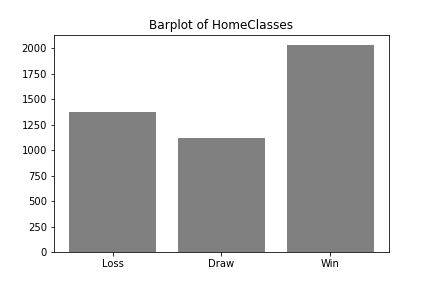
\includegraphics[width=0.6\textwidth]{histogram_of_HomeClasses.png}
	\caption{Bar plot of match outcome for home team.}
	\label{fig:BarPlot}
\end{figure}

\subsection{Treatment}

In the dataset there are two variables indicating the squad's market value of the home and away team, respectively. In figure \ref{fig:TimeSeries} below, the evolution of each observed team's market value between 2006/07 and 2020/21 is plotted. Although most teams seem to possess a relatively constant market value of around \euro{}100 to \euro{}200 million, the trend seems to be slightly increasing after the 2017/18 season. Interestingly, it can also be observed that in the latest season there is a slight dip in all teams' market values. This can be attributed to the coronavirus pandemic, which drastically hurt the profitability of the soccer industry and led to many players loosing value. There are also a few outliers from the majority of the league, such as Bayern Munich and Borussia Dortmund, who consecutively have had a higher market value than the rest of the league. It may be worthwhile controlling for such extreme outliers in a later stage of the analysis.

\begin{figure}[ht]
	\centering
	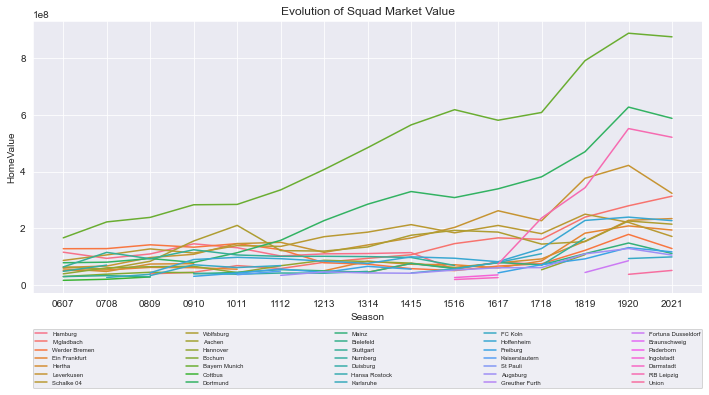
\includegraphics[width=1\textwidth]{MarkVal2.png}
	\caption{Evolution of squad market values.}
	\label{fig:TimeSeries}
\end{figure}

In order to directly address the research question, these variables were recoded into dummies which describe whether the home squad had a higher market value than the away side.

\begin{table}[ht]
\centering
	\begin{tabular}{lll} \toprule {}
	  &     Share &   Obs \\
	HomeHigherVal &           &       \\  \midrule
	0             &  0.499 &  2258 \\
	1             &  0.501 &  2269 \\  \bottomrule
	\end{tabular}
\caption{Distribution of treatment variable}
\label{tab:treatmentDist}
\end{table}

From table \ref{tab:treatmentDist} it can be seen that the share of observations in which the home team is valued more highly (and vice versa) are perfectly balanced with a share of 0.5 each. The observations in each category of the dummy variable are almost identical, too. This arises from the fact that the random sub sample of the data set has an almost perfectly balanced share of first-leg and second-leg games (home vs. away matches) per season per team. For each season, 17 first- and second-leg games are observed for each team, thus a complete season of 34 matches in total per team. Only in the latest season, 2020/21, 13 Home and 14 Away games are observed per team. This balance implies that each team is equally well represented in the data set as the home and the away team, thus leading to the equal share shown in table \ref{tab:treatmentDist}. The equal share of matches observed per season is also evident from the equal mean across all seasonal dummy variables in table \ref{tab:SummaryStatTab}.

The table \ref{tab:treatmentOutcome} below shows the mean of treatment, with respect to the three match outcome classes. Although this is only an indication of correlation, not causation, we can see that the share of observations for which the home team had a greater market value increases from 0.334 when the Home team looses, to 0.491 when they draw, to 0.62 when they win. This indicates that home teams who are more expensive tend to win more home games, as the unconditional probability of winning is almost twice as high as loosing. In Section 4 this report tests whether this trend still holds when controlling for potential confounders.

\begin{table}[ht]
\centering
	\begin{tabular}{lll}
	\toprule
	{} & HomeHigherVal &   Obs \\
	HomeClasses &               &       \\
	\midrule
	Loss          &         0.334 &  1378 \\
	Draw           &         0.491 &  1117 \\
	Win           &          0.62 &  2032 \\
	\bottomrule
	\end{tabular}
\caption{Mean of treatment for match outcome}
\label{tab:treatmentOutcome}
\end{table}

\subsection{Control Variables}

As the research question and match outcome are encoded from the perspective of the home team, most variables were recoded to represent the difference between the home and away side. These include the difference in GDP, unemployment rate, and TV revenues. Furthermore, we decided to include match specific statistics such as shots taken, corners and yellow/red cards received, as previous literature has shown that such variables both have an effect on the match outcome as well as the market value of players \cite[p. 614]{muller2017}. Due to such possible confounding, we included these in our model specification. Possible issues regarding the exogeneity assumption of confounders, due to the possibility of treatment having an effect on match specific characteristics, will be discussed in the \textit{Discussion} section of this paper.

A full list of covariates used and their corresponding summary statistics can be found in Table \ref{tab:SummaryStatTab} below. These include the dependent variable (HomeHigherVal), treatment (HomeClasses), as well as all  covariates used for the explained model specification.

As can be seen in table \ref{tab:SummaryStatTab}, the data shows no anomalies. There are no missing values for any variables and all dummy variables have an appropriate range and unique values, as should be expected. Furthermore, some variables also have a rounded mean of 0.00. For the differenced variables this is given by the set up of the dataset with first- and second-leg for each season. Further, the mean for dummy variables such as "SecondNewCoachHome" and "HomeRelegated" (and all other associated dummy variables of those) are also zero. Thus, the sample observes a very small amount of observations for which these dummy variables equal 1. Thus, any statistical inference on these dummy variables would not be possible as the available sample size would be too small.

Regarding the treatment variable, however, it can be seen that the share is very balanced as discussed in Section 2.2. The mean of the dependent variable, \textit{HomeClasses}, is 1.1, further showing that the classes are not perfectly balanced as previously shown in Figure \ref{fig:BarPlot}, as home teams tend to win with the same frequency as the combined frequency with which they draw or loose.

\begin{table}[h!]
	\centering
	\scalebox{0.65}{
			\begin{tabular}{lrrrrrrrr}
				\toprule
				{} &   MEAN &    VAR &   STD &    MAX &    MIN &  MISSING &  UNIQUE &  COUNT \\
				\midrule
				HomeClasses    &    1.1 &    0.7 &   0.9 &    2.0 &    0.0 &        0 &       3 &   4527 	\\
				HomeHigherVal  &    0.5 &    0.3 &   0.5 &    1.0 &    0.0 &        0 &       2 &   4527 \\
				Attendance     &   40.3 &  370.6 &  19.3 &   81.4 &    0.0 &        0 &    2009 &   4527 \\
				HomeShots      &   14.4 &   26.5 &   5.1 &   36.0 &    1.0 &        0 &      36 &   4527 \\
				AwayShots      &   11.8 &   22.3 &   4.7 &   33.0 &    0.0 &        0 &      32 &   4527 \\
				HomeFouls      &   14.8 &   22.4 &   4.7 &   33.0 &    2.0 &        0 &      32 &   4527 \\
				AwayFouls      &   15.8 &   25.7 &   5.1 &   35.0 &    1.0 &        0 &      35 &   4527 \\
				HomeCorners    &    5.5 &    8.7 &   2.9 &   20.0 &    0.0 &        0 &      21 &   4527 \\
				AwayCorners    &    4.4 &    6.3 &   2.5 &   14.0 &    0.0 &        0 &      15 &   4527 \\
				HomeYellows    &    1.6 &    1.5 &   1.2 &    8.0 &    0.0 &        0 &       9 &   4527 \\
				AwayYellows    &    2.0 &    1.6 &   1.3 &    7.0 &    0.0 &        0 &       8 &   4527 \\
				HomeReds       &    0.1 &    0.1 &   0.3 &    2.0 &    0.0 &        0 &       3 &   4527 \\
				AwayReds       &    0.1 &    0.1 &   0.3 &    3.0 &    0.0 &        0 &       4 &   4527 \\
				AvgAgeHome     &   24.6 &    0.8 &   0.9 &   27.1 &   22.1 &        0 &     356 &   4527 \\
				StdvAgeHome    &    4.3 &    0.3 &   0.5 &    5.8 &    2.8 &        0 &     420 &   4527 \\
				AvgAgeAway     &   24.6 &    0.8 &   0.9 &   27.1 &   22.1 &        0 &     360 &   4527 \\
				StdvAgeAway    &    4.3 &    0.3 &   0.5 &    5.8 &    2.8 &        0 &     421 &   4527 \\
				BothHome       &    0.1 &    0.0 &   0.1 &    0.3 &    0.0 &        0 &      93 &   4527 \\
				BothAway       &    0.1 &    0.0 &   0.1 &    0.3 &    0.0 &        0 &      93 &   4527 \\
				AvgHeightHome  &  183.6 &    1.0 &   1.0 &  186.9 &  181.3 &        0 &     306 &   4527 \\
				StdvHeightHome &    6.5 &    0.5 &   0.7 &    8.5 &    4.3 &        0 &     359 &   4527 \\
				AvgHeightAway  &  183.6 &    1.0 &   1.0 &  186.9 &  181.3 &        0 &     306 &   4527 \\
				StdvHeightAway &    6.5 &    0.5 &   0.7 &    8.5 &    4.3 &        0 &     359 &   4527 \\
				HomeChampion   &    0.0 &    0.0 &   0.1 &    1.0 &    0.0 &        0 &       2 &   4527 \\
				AwayChampion   &    0.0 &    0.0 &   0.1 &    1.0 &    0.0 &        0 &       2 &   4527 \\
				HomeRelegated  &    0.0 &    0.0 &   0.0 &    1.0 &    0.0 &        0 &       2 &   4527 \\
				AwayRrelegated &    0.0 &    0.0 &   0.0 &    1.0 &    0.0 &        0 &       2 &   4527 \\
				DiffGDP        &   -0.0 &    0.1 &   0.3 &    0.8 &   -0.8 &        0 &    3567 &   4527 \\
				DiffUnempl     &    0.0 &   25.7 &   5.1 &   17.4 &  -17.4 &        0 &     768 &   4527 \\
				DiffTV         &   -0.0 &  106.8 &  10.3 &   41.8 &  -41.8 &        0 &    2167 &   4527 \\
				Season\_0607    &    0.1 &    0.1 &   0.3 &    1.0 &    0.0 &        0 &       2 &   4527 \\
				Season\_0708    &    0.1 &    0.1 &   0.3 &    1.0 &    0.0 &        0 &       2 &   4527 \\
				Season\_0809    &    0.1 &    0.1 &   0.3 &    1.0 &    0.0 &        0 &       2 &   4527 \\
				Season\_0910    &    0.1 &    0.1 &   0.3 &    1.0 &    0.0 &        0 &       2 &   4527 \\
				Season\_1011    &    0.1 &    0.1 &   0.3 &    1.0 &    0.0 &        0 &       2 &   4527 \\
				Season\_1112    &    0.1 &    0.1 &   0.3 &    1.0 &    0.0 &        0 &       2 &   4527 \\
				Season\_1213    &    0.1 &    0.1 &   0.3 &    1.0 &    0.0 &        0 &       2 &   4527 \\
				Season\_1314    &    0.1 &    0.1 &   0.3 &    1.0 &    0.0 &        0 &       2 &   4527 \\
				Season\_1415    &    0.1 &    0.1 &   0.3 &    1.0 &    0.0 &        0 &       2 &   4527 \\
				Season\_1516    &    0.1 &    0.1 &   0.3 &    1.0 &    0.0 &        0 &       2 &   4527 \\
				Season\_1617    &    0.1 &    0.1 &   0.3 &    1.0 &    0.0 &        0 &       2 &   4527 \\
				Season\_1718    &    0.1 &    0.1 &   0.3 &    1.0 &    0.0 &        0 &       2 &   4527 \\
				Season\_1819    &    0.1 &    0.1 &   0.3 &    1.0 &    0.0 &        0 &       2 &   4527 \\
				Season\_1920    &    0.1 &    0.1 &   0.3 &    1.0 &    0.0 &        0 &       2 &   4527 \\
				\bottomrule
			\end{tabular}}
		\caption{Table of descriptive summary statistics of all variables.}
		\label{tab:SummaryStatTab}
\end{table}

% \begin{adjustbox}{totalheight=\textheight-2\baselineskip, width=\textwidth}
% \end{adjustbox}

%-------------------------------------------------------------------------------

\section{Methods}

In this analysis two different estimators were used. First, an ordinal logistic regression was performed that minimized a margin based loss function. Secondly, an ordered forest was used to also measure the marginal effect of higher valuation on success in a non-parametric model. The performance of these approaches in a predictive sense were then measured by two slightly different version of the mean squared error (MSE) and the classification accuracy (CA).

%------------------------------------------------
%	Logistic Regression
%------------------------------------------------

\subsection{Ordinal Logistic Regression}

For starters a logit model was used to estimate the response probabilities and in the end derive the marginal effect of a higher valuation of the home team on success. An ordered logit model assumes an ordered response random variable that corresponds to the respective classes in the analysis. In this case, this ordered random variable is given by the recoded covariate \textit{HomeClasses}. This covariate can have three different values. Namely, 0, 1, and 2, which correspond to a loss of the home team, a draw, and a win of the home team. Assuming now a latent linear model

$$
Y^{*} = X\beta + U, \quad U | X = x \sim F(0, \sigma^2)
$$

and a set of unknown thresholds

$$
\alpha_1 < \alpha_2
$$

the observations can be classified into the ordinal classes \textit{loss}, \textit{draw}, or \textit{win}. The classification is done according to the following criteria:

\begin{align*}
	Y &= 0 \quad \text{if } Y^{*} \leqslant \alpha_1, \\
	Y &= 1 \quad \text{if } \alpha_1 < Y^{*} \leqslant \alpha_2, \\
	Y &= 2 \quad \text{if } Y^{*} > \alpha_2.
\end{align*}

Further, assuming a logistic distribution for the probabilities, the cumulative distribution function of a logistic distribution can be used to compute the corresponding choice probabilities. \cite[p. 36f]{lechner2021}

Using this logit model it can be seen that the coefficients and the thresholds have to be estimated. To estimate these parameters a maximum margin loss function was used. This objective function implies that it predicts the class correctly including a margin. In general, this loss function can be expressed by \cite{rennie2005}:

$$
\text{loss}(y^{*}; y) = \sum f \left(s(l; y) \cdot (\alpha - y^{*})\right)
$$

\vspace{12pt}

where $s(l; y) = \begin{cases}-1 \quad \text{if } l \leqslant y \\ 1 \quad \text{if } l > y\end{cases}$, $l = \begin{bmatrix}0 \\ 1\end{bmatrix}$, and $f(z) = \log(1 + \text{exp}(-z))$.

\vspace{12pt}

Minimizing this objective function corresponds to maximizing the geometrical margin $M = \frac{1}{|\beta|}$ around the hyperplane, while minimizing the number of misclassified training points with a margin of at least $M$ \cite{rennie2005}.

For starters a simple gradient descent algorithm was used to optimize the logarithmic objective function. Gradient descent algorithms generally are easy to implement and often perform quite well. To find the minimum of the objective function the algorithm starts at some arbitrary values for the coefficients and the thresholds. Then the values will be iteratively updated by the learning rate $\gamma$ times the gradient. Since the gradient goes to zero when approaching the minimum, the coefficients and thresholds will also converge to their optimal values \cite[p. 113f]{chong2013}.

$$
x^{(k + 1)} = x^{(k)} - \gamma \cdot \nabla f(x^{(k)})
$$

The main parameters in a gradient descent algorithm that have to be defined are the learning rate and number of iterations. The learning rate defines the size of updating. Meanwhile, the number of iterations defines the number of times the coefficients and thresholds will be updated. To find the optimal values of the coefficients and thresholds in this analysis a learning rate of $\gamma = 10^{-8}$ was used and the number of iteration was chosen to be $10'000$.

In general, the gradient descent algorithm is known to depend strongly on the choice of the learning rate and the arbitrary starting point. To check the performance of the gradient descent algorithm, the objective function was also optimized using a Broyden-Fletcher-Goldfarb-Shanno (BFGS) algorithm, which was implemented by using the Python package \textit{SciPy}\footnote{For further reading regarding \textit{SciPy} one can check out its documentation \cite{scipy2021}.}. The results of these different optimization approaches are discussed below.

%------------------------------------------------
%	Ordered Forest
%------------------------------------------------

\subsection{Ordered Forest}

An ordered random forest model that predicts the probabilities of the different classes is based on a binary random forest regressions. A binary forest model is a non-linear and non-parametric model that seeks to minimize mean squared errors in each sub sample. In our model, the forest contains 1'000 trees by default. Thirty percent of the covariates are randomly drawn without replacement. By using a bootstrapping to build each tree the correlation between the trees is reduced and the increase in the variance is limited \cite[p.588]{hastie2009}. In each node of a tree there is a threshold of the corresponding covariate to minimize the total MSE and a minimum amount of 5 observations is defined to deepen the tree sufficiently. In conclusion, a random forest estimator can be considered as a flexible method to estimate the relationship between an outcome variable and multiple covariates.

After building a random forest, an observation can be inserted to predict the probability of it belonging to either class 0 or 1. The observation goes through the first tree and moves down to different nodes depending on whether it is above the respective threshold or not. Then a tree forecasts the outcome value. Subsequently, the observation iterates through all the trees and gets a a list of values. Then, the average of the values defines the estimated conditional probability that it belongs to the corresponding class.

Based on binary models estimated by the random forests, an ordered random forest model can be established to deal with multiple classes \cite[p.7]{lechner2019random}. To simplify the procedure, assume that there are three classes, as for example 1, 2, and 3.  Then, the outcome variable needs to be divided into three columns in an ascending order such that they can be represented as dummy variables in the next step. Further, these columns can be used to iterate through the binary random forest for the predictions.

For the first iteration, keep the class 1 dummy and turn the other 2 dummies into zero and combine them to form a new outcome variable for the forest prediction and obtain the first set of probabilities. For the second iteration,  keep the first two dummies and only turn the class 3 dummy into zero. Then, combine them to attain the second set of probabilities. The number of iterations correspond to the number of classes minus 1.

The next step is replicating the results to create two sets of probabilities. The first set has a column of 1 at the end column while the second set has a column of 0 at the first column. Eventually, take the difference of the cumulative probabilities to isolate the respective class probabilities $\hat{P}_{m,i} = \hat{Y}_{m,i} - \hat{Y}_{m-1, i}$ \cite[p.7]{lechner2019random}. One also needs to conduct a normalization by dividing the probabilities with the sum of probabilities in its corresponding row.

$$
\text{Culmulative Probabilities} = \begin{bmatrix}
P_{1,1}\quad P_{(1,2),1}\\
P_{1,2}\quad P_{(1,2),2}\\
\vdots\quad \vdots\\
P_{1,n}\quad P_{(1,2),n}\\
\end{bmatrix}
\qquad
\text{Isolated Probabilities} =
\begin{bmatrix}
P_{1,1} & P_{2,1} & P_{3,1}\\
P_{1,2} & P_{2,2} & P_{3,2}\\
\vdots & \vdots & \vdots\\
P_{1,n} & P_{2,n} & P_{3,n}\\
\end{bmatrix}
$$

The resulting probabilities will then be used to compute the marginal effects for the causal analysis, the MSE, and the CA for predictive performance tests later on.

%-------------------------------------------------------------------------------

\section{Results}

\subsection{Marginal Effects}

The following results regarding the estimated marginal effects were obtained using the whole dataset, such that all observations were considered and the sample size can be maximized. While the ordered random forest only generates predictions without any functional form, ordered logit is a parametric model with a specified functional form, where for each covariate a coefficient is estimated. It is important to mention that these coefficients are not informative of the size of the causal effects of the treatment on the outcome variable. Generally, one can only get the direction of the effect by looking at the coefficients itself. To further get the size of the effect, how the conditional probabilities regarding the outcome changes in response to a change in the covariates, one needs to estimate the marginal effects.

The marginal effects are reported in this analysis using the mean marginal effects, which means that the marginal effect for each observation gets computed and then one computes the average. This approach was used instead of the marginal effect at the mean, due to the fact that the mean of some covariates (e.g. the season dummies) do not have a clear interpretation \cite[p.310]{bartus2005}.
$$
\text{Mean Marginal Effects:} \qquad \hat{\delta}_j = \hat{\beta}_j \frac{1}{N} \sum^N_{i=1} g(x_i \hat{\beta})
$$

The results in table \ref{tab:MeanMarg} highlight the mean marginal effects of the higher market value of the home team on the outcome of the games.  Intuitively one might think that higher home team values lead to a higher chance of winning, an ambiguous chance of drawing, and a lower chance of losing. Hence, the positive sign in the class with 3 points and the negative sign for the class with 0 point presented in the results table below are consistent with one's expectations. Further, one can note that the sum of the mean marginal effects is equal to zero. This is due to the fact that an increase in probability of one class is compensated by a decrease in another class.

As described in the methods chapter, two different optimization algorithms were used to estimate the ordered logit model. First, a gradient descent algorithm was used. Since this optimization algorithm sensitively react on the specification of the learning rate, a BFGS optimization procedure was used as a benchmark. The two optimization algorithms lead to a different value of the objective function at the optimal level. While the gradient descent algorithm leads to an objective of 7'358.27, the BFGS algorithm reaches even a smaller objective of 5'211.61. Which would suggest that the BFGS optimizer has outperformed the gradient descent algorithm with respect to the specifications used. Nevertheless, the mean marginal effects are rather similar.

\begin{table}[ht]
\centering
	\begin{tabular}{lrrr}
	\toprule
	{} &   0 point &   1 point &  3 points \\
	\midrule
	OLogit - GD & -0.076 & -0.006 & 0.082 \\
	OLogit - BFGS & -0.063 & -0.011 & 0.074 \\
	ORF    & -0.061 &  0.009 &  0.052 \\
	\bottomrule
	\end{tabular}
	\caption{Mean marginal effects of higher home value}
	\label{tab:MeanMarg}
\end{table}

Subsequently, the marginal effects are multiplied by the corresponding numbers of points to compute the average number of extra points the home team can expect if it has a higher market value. Table \ref{tab:numpoints} underlines that a home team could expect 0.241 extra points from a match if it is more expensive than the rival team based on an ordered logit model using gradient descent. By using a BFGS-algorithm to optimize the objective function the extra points get slightly reduced to 0.212. Lastly, considering the random forest estimator, the model suggests an expected value of 0.165.

\begin{table}[ht]
\centering
	\begin{tabular}{llll}
	\toprule
	{} &    OLogit - GD & OLogit - BFGS & ORF \\
	\midrule
	Number of additional points & 0.241 & 0.212 &  0.165 \\
	\bottomrule
	\end{tabular}
	\caption{Number of extra points to expect, if the home team is more expensive.}
	\label{tab:numpoints}
\end{table}


\subsection{Prediction}

In order to examine our estimators the accuracy of predictions is evaluated. Therefore, the data frame is randomly split into a training (80\%) and a test set (20\%)\footnote{The training and test split was performed for each season, such that the seasons are weighted equally in the respective sub samples.}. All the estimators are trained using the training set. The conditional probabilities are then predicted separately for each estimator using the test set. Next, the prediction accuracy is calculated with the following three measures.

$$MSE_1 = \frac{1}{N} \sum_{i = 0}^N \sum_{j=1}^J (I(Y_i = j) - \hat{P}[Y_i = j \mid X_i = x])^2$$
$$MSE_2 = \frac{1}{N} \sum_{i = 0}^N (Y_i  - \sum_{j=1}^J j * \hat{P}[Y_i = j \mid X_i = x])^2$$
$$CA = \frac{1}{N} \sum_{i = 0}^N I(Y_i  = \hat{Y_i}) , \text{ if } \hat{Y_i} \text{ is the class with the highest probability.}$$

The results are shown in table \ref{tab:predictions}. The classification accuracy ranges from 43.9\% to 52.7\%. Which would suggest that the ordered random forest outperforms the ordered logit model in a predictive sense considering the classification accuracy. This also holds to be true when comparing the different estimators according to the MSE.

\begin{table}[ht]
\centering
	\begin{tabular}{lrrr} \toprule {}
	  &     $MSE_1$ &  $ MSE_2$ & $CA$ \\
	  \midrule
	OLogit - GD &   0.783 & 1.022 & 0.439 \\
	OLogit - BFGS &   1.025 & 1.393 & 0.487 \\
	ORF &     0.586  & 0.646 & 0.527 \\  \midrule
	\bottomrule
	\end{tabular}
\caption{Prediction performance for both estimators.}
\label{tab:predictions}
\end{table}

%-------------------------------------------------------------------------------

\section{Discussion}

\subsection{Causal Effects}
A home team in the German Bundesliga, given that it has a higher market value than the away team, can expect to score more points on average. At least this was shown in the chapter before, when the mean marginal effects were estimated. But do these effects reflect causality or only spurious correlation? In this section, the identifying assumptions for a selection-on-observables research design and the necessary assumptions for both estimators are discussed to answer this question.

\subsubsection*{Assumptions}

For a causal effect to be identified, four assumptions should be met in this research design for any estimator used: Conditional independence, common support, exogeneity of confounders, and the stable unit treatment value assumption \cite[p. 16f]{lechner2021_da2}.

First, conditional independence is given if all variables that the model conditions, takes every covariate that jointly influences the outcome and the treatment variable into account. One might argue that the model should also control for the total amount of passes or the total amount of distance covered by each team for a given match. This is due to the fact that one might assume that these two variables influence the outcome of the game and at the same time have a positive effect on the market value of the players, thus also the teams' value. Nevertheless, this report argues in line with \citeA{muller2017}, that the models control for the most important confounders and hence one might assume that the conditional independence assumption holds.

Second, common support may be assumed to hold given by the structure of the dataset. In each but the last season, every team plays against every other team two times. Once as the home team and once as the away team. So, for every given value of the confounding variables, once the home team has a higher value and once the away team has a higher value. Hence, this assumption is assumed to hold.

Exogeneity of confounders is the third identifying assumption. In order for this assumption to hold the covariates used cannot be influenced by the treatment in a similar way to the outcome variable. If this assumption does not hold the coefficients of the models converge towards zero and no effect would be predicted. Here, one could argue that the market value influences the match related variables in the same way as it has an impact on the outcome of the game \cite[p. 614]{muller2017}. Therefore, one might conclude that the exogeneity assumption may not hold.

Lastly, the stable unit treatment value assumption defines that there should not be relevant interactions between treatments. So the fact that team \textit{a} is more expensive than team \textit{b} should not have any effect on the match outcome between team \textit{b} and team \textit{c}. Since the treatment is given by comparison of the two teams in a match and due to the fact that multiple characteristics of the players come into play when defining the market value, it can be assumed that also this last assumption may hold.

Next to the identifying assumptions one needs to consider the model specific assumptions. The logistic regression assumes a latent linear model and a logistic distribution of the error terms and probabilities \cite[p. 519]{cameron}. Assuming that these two assumptions hold, the logistic regression is a consistent estimator of the corresponding causal effect. On the other hand, the ordered random forest belongs to the class of non-parametric estimators and hence, does not rely on any distributional assumptions \cite[p. 1]{lechner2019random}.

Further, both models assume that the underlying dependent variable has an ordinal structure, which is indeed the case in this analysis. The logistic regression in particular also assumes that the outcomes behave in an ordinal fashion with respect to each covariate \cite{regrmodels}. This assumption then implies the single crossing property with relation to the mean marginal effects. It can be argued that this ordinal relationship between the outcome and the covariates might hold in this context. Next, multicollinearity can also pose an issue. Hence, one season variable was dropped and it was checked using a correlation matrix that no perfectly collinear covariates were included in the model.

%Finally, the ordinal logistic regression also needs a parallel regression assumption. This is the case, because the logit model only consists of one set of coefficients. Generally this implies that the relationship between all outcome groups has to be the same. \hl{source} have only found thins about this in forums. not in a single book. and it seems that it is quite the same as the single crossing property. it basically says that the odds between all categories are the same.

In conclusion, this report argues that all the assumptions except the exogeneity of confounders assumption may hold. Thus, this implies that the computed marginal effects may converge towards zero. One might therefore conclude that the direction of the effect could be identified as causal, but not the size of the effect.


\subsection{Predictive Performance}

Given the values presented in table \ref{tab:predictions}, it is possible to conclude that both the ordered forest and the two versions of the ordered logit model perform similarly well in terms of the MSE and classification accuracy.  Although the GD ordered logit predicts 44\% of the classes correctly, both the BFGS logit and ordered random forest predict approximately 50\% of all classes correctly. Interestingly, with regards to the MSE the ordered forest performs slightly better with a MSE of around 0.6, whereas the two logit models each have a $MSE_1$ ranging from 0.8 to 1.0, respectively an $MSE_2$ ranging from 1.0 to 1.4. Furthermore, although the BFGS logit has a slightly higher CA, its MSE values are consistently higher than those of the GD logit. This may be explained by the fact that the BFGS logit model minimizes a maximum margin loss function. Thus, the BFGS logit aims to optimize the CA, leading to a situation in which the gradient descent logit can perform worse in terms of CA, but is better in terms of MSE. A further issue is that the GD and BFGS logit do not predict the outcome class 1 (match outcome is a draw) in the sample. The ordered random forest, on the other hand, predicts this class. This is not surprising since it is a more flexible approach in estimating the outcome classes. Also, outcome class 1 has the least observations.



\subsection{Robustness check}

As shown in the data section, the data incorporates a time dimension and several outliers. Two robustness checks are therefore implemented to control for heterogeneity and time effects.

First, referring to the earlier discussion, the market values of the football teams experience an upward trend but are overall converging, in line with the random selection assumption for the causal analysis. However, two outliers stand out from the figure: Bayern Munich and Dortmund. They demonstrate substantially higher market values than the other teams in most seasons. Eliminating the outliers could lead to a more general estimate of the treatment effect. The new results show that a more valuable home team should expect 0.16 and 0.11 extra points using ordered logit and ordered forest, respectively. This decline in the number of points is noticeable but does not change the direction of the estimates. %This could confirm the previous assumption that the two outliers exist in our model, since they are almost always more expensive than the away team when playing at their home stadiums.

%First, referring to the earlier discussion, the market values of the football teams experience an upward trend but are overall converging, in line with the random selection assumption for the causal analysis. However, two outliers stand out from the figure: Bayern Munich and Dortmund. They demonstrate substantially higher market values than the other teams in most seasons, threatening to compromise the random assumption. For example, if Bayern Munich is the home team, it could expect more points than when Aachen is the home team. So eliminating the outliers could lead to a more general estimate of the treatment effect. The new results show that a more valuable home team should expect 0.16 and 0.11 extra points using ordered logit and ordered forest, respectively. This decline in the number of points is noticeable but does not change the direction of the estimates. This could confirm the previous assumption that the two outliers exist in our model, since they are almost always more expensive than the away team when playing at their home stadiums.

Second, the yearly changes of the marginal effects are computed to show whether they are consistent with the main results. The goal here is to exploit the panel structure of the data. This check illustrates in figure \ref{fig:ATEslogit} significant jumps and drops in certain years but should be taken with caution due to the small subsample sizes for each season.

Figure \ref{fig:ATEslogit} shows the mean marginal effects of higher home team value on the three outcome classes estimated by a logit model. It highlights that the probability of the middle class is always between the other two classes due to the monotonicity restriction imposed by the ordered logit model. The other two probabilities are symmetric because the mean marginal effects remain close to zero and the sum of the effects must be equal to zero as well. Therefore, this check illustrates the drawback of the inflexibility of the logit model, even though it might not give reliable estimates of ATEs due to the small sub sample sizes. In contrast, the ordered forest model allows the middle class probability to transcend the other two classes and is therefore more flexible.  In short, ordered logit may not be suitable for small sample sizes but is plausible when the sample size is sufficiently large, while ordered forest only demonstrates limited volatility regardless of the sample sizes.

\begin{figure}[ht]
\centering
\begin{minipage}{.5\textwidth}
  \centering
  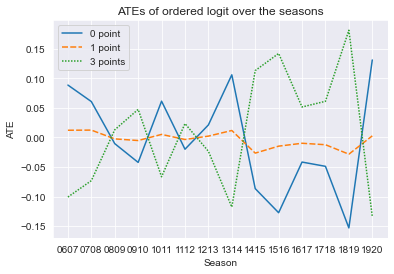
\includegraphics[width=1\linewidth]{ATEs_logit.png}
  \caption{ATEs of ordered logit model.}
  \label{fig:ATEslogit}
\end{minipage}%
\begin{minipage}{.5\textwidth}
  \centering
  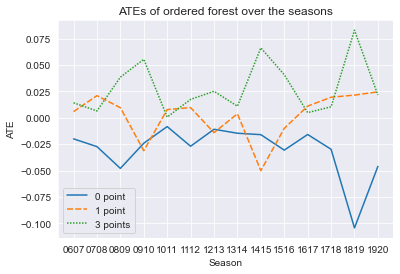
\includegraphics[width=1\linewidth]{ATEs_orf.png}
  \caption{ATEs of ordered random forest.}
  \label{fig:ATEsorf}
\end{minipage}
\end{figure}

%-------------------------------------------------------------------------------

\section{Conclusion}

In this analysis data from the German Bundesliga was used to estimate the average points the home team can expect, if it has a higher market value than the away side. The data considers the first and second half of the season for the seasons 06/07 to 20/21. This suggests that the treatment, being of higher market value, is evenly distributed. Combined with a selection of covariates an ordinal logistic regression and an ordered forest is trained. Overall, our results show that the home team, if it has a higher market value than its opponent, could expect 0.212 points more according to the logit model using a BFGS optimization algorithm, or 0.165 points more according to the ordered random forest.

In general, the ordinal logistic regression and the ordered forest both predict a positive mean marginal effect of having a higher market value on winning the match. Further, by splitting the data in a train and test split the prediction performance can be measured out-of-sample. Here, two different measures were used. First, two slightly different specification for the mean squared error were computed and secondly, the classification accuracy was derived. Based on the prediction performance the data suggests that the ordered forest performs a bit better than the ordinal logistic regression regarding both performance measures.

If these estimators capture a true causal effect of higher market value on the outcome of the game depends on the credibility of its identifying assumptions. This report argues, that the conditional independence assumption may be assumed to hold. On the other hand, one could have an endogeneity problem. Thus, the estimated effects might be biased towards zero. Therefore, one might conclude that there is a positive causal effect and the home team can expect a positive amount of points by solely having a higher market value. Although, the marginal effects seem to be robust regarding outliers, this analysis cannot credibly determine the specific size of the effect.

\pagebreak

%-------------------------------------------------------------------------------

% remove page numbering
\pagenumbering{gobble}

% Display references
\bibliography{refSelfStudy} % corresponds to the file refSelfStudy.bib

\end{document}
